\section{Le nettoyage de données, data cleaning, data cleansing, data scrubbing}

Le manque de qualité des données coûte 600 milliards de dollars à l’économie américaine chaque année. (Interaction between Record Matching and Data Repairing, Wenfei Fa et ali., 2011).\\
Ce constat alarmant montre la nécessité de s’intéresser au problème de la qualité des données, afin de le corriger en amont (faire la prévention, par le biais de M.D.M. par exemple), mais aussi en aval (de la correction, par le biais de “data cleaning”).
Le data cleaning est un sujet d’étude finalement assez récent, mais qui semble prometteur, puisque le marché du data cleaning est en hausse de 17%, alors que le reste du marché de l’informatique est “seulement” en hausse de 7%.\\
Une vrève définition de ce qu’est le data cleaning s’impose : l’objectif du data cleaning est de supprimer les erreurs et les incohérences d’un base de données afin d’améliorer la qualité des données.\\
Cependant, avant d’aborder plus avant le sujet du data cleaning à proprement parler, il est nécessaire d’aborder le sujet de la qualité de données. Comprendre l’origine et la diversité des problèmes de la qualité des données est nécessaire pour correctement aborder le sujet du data cleaning.\\
Nous verrons donc dans un premier temps quels peuvent être les différentes origines de la mauvaise qualité de données.\\
Les données fournies au système de nettoyage de données sont la plupart du temps d’origines diverses, et elle proviennent notamment souvent de bases de données différentes.\\
Ces origines diverses sont à l’origine de plusieurs problèmes concernant la qualité des données.\\
Voici un schéma récapitulant brièvement les différents problèmes concernant la qualité des données (source : Fig. 2, Data Cleaning: Problems and Current Approaches, Erhard Rahm et al.)

\begin{figure}[H]
\begin{center}
 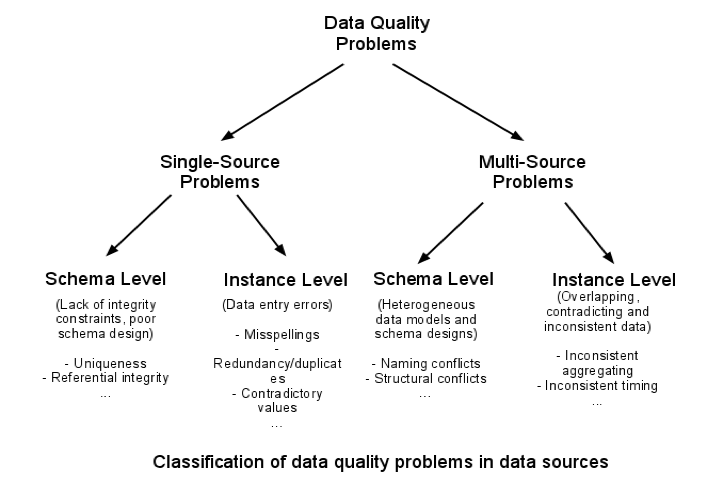
\includegraphics[scale=0.5]{ClassificationData.png}
  \caption{}
\end{center}  
\end{figure}

Nous voyons donc qu’il est possible de séparer les problèmes de qualité de données selon deux origines principales :
\begin{itemize}
\item[-]les problèmes internes à une source de données unique
\item[-]les problèmes liés à des données ayant des sources multiples
\end{itemize}
Il est aussi possible de distinguer deux autres sous-catégories de problèmes liés à la qualité des données :
\begin{itemize}
\item[-]les problèmes liés au modèle de données (le schéma de données)
\item[-]les problèmes liés aux données elles-mêmes (incohérences au niveau des données entre autres)
\end{itemize}
Nous aborderons dans un premier temps les problèmes liés aux sources de données uniques.\\
Les problèmes liés aux modèles de données sont principalement des problèmes liés à de mauvaises définitions du modèle données (violation de contraintes d’intégrité, unicité non respectée, valeurs illégales, etc....).\\
Les problèmes liés aux données elles-même sont quant-à-eux un peu plus variés. Il peut s’agir de problèmes liés à des valeurs manquantes ou erronées (fautes de frappes, d’orthographe, abréviations, erreurs de champs, etc...), à des incohérences entre plusieurs valeurs d’une même données (exemple : ville Paris, et code postal 42000), ou encore à des incohérences entre différentes données (données enregistrées plusieurs fois - et éventuellement de manière légèrement différentes, données incohérentes entre-elles).\\
Il est évident que ces problèmes se retrouvent souvent combinés entre-eux, et ainsi créer des problèmes bien plus complexes.\\
Les meilleurs moyens de résoudre (la plupart) de ces problèmes consiste à introduire un modèle de données fiable et cohérent laissant le minimum de libertés aux données, évitant ainsi un maximum d’erreurs.\\
Nous verrons ensuite les problèmes liés aux sources de données multiples. Ceux si sont sensiblement aggravés en comparaison des problèmes liés aux sources de données uniques, et sont bien plus nombreux.\\
Les problèmes liés aux modèles de données sont assez nombreux. Tout d’abord, l’un des problèmes provient du fait que les schémas de données des multiples sources sont différents.\\
Il faut donc dans premier temps convertir toutes les sources de données vers un schéma unique. Il faut à ce moment là définir deux autres types de problèmes : 
\begin{itemize}
\item[-]les problèmes de nommage : un même nom d’attribut correspondant à plusieurs types d’attributs différents (homonymes, par exemple id) ou plusieurs noms d’attribut correspondant finalement à unique type d’attribut (synonymes, name et nom par exemple).
\item[-]les problèmes structurels : ce sont des problèmes dus à des représentations de la même donnée de manières différentes (pas le même types de données - bool, string -, contraintes d’intégrité différentes, etc...).
\end{itemize}
Les problèmes liés aux données elles-mêmes sont assez similaires aux mêmes problèmes liés aux sources de données uniques (duplicité des données, incohérences, etc...), combinés aux problèmes de représentation différentes des données. Même si ces problèmes de représentation ne semble pas toujours présents au premier abord (même nom d’attributs, même types de données) il faut rester prudent quant à l’exploitation des résultats (interprétation des données différentes par exemple - prix en dollar ou en euro -...).\\
La principale difficulté posée par la présence de sources de données multiples est en fait la difficulté de déterminer quelles sont les données se référant à une même entité réelle.\\
Si la plupart des problèmes liés aux modèles de données peuvent - et doivent dans la mesure du possible - être corrigés en amont, il n’est pas toujours possible de faire de même concernant les problèmes liées aux données elle-mêmes. C’est donc principalement sur ce problème que s’attardent les solutions de data cleaning.\\
Pour résumer, les données, une fois présentées via le même schéma de données, présentent encore des problèmes de cohérence entre-elles.\\
Il faut donc être capable de déterminer ces incohérences et des les corriger. Ce problème peut se décomposer en deux sous-problèmes principaux :
\begin{itemize}
\item[-]déterminer les données se référant à une unique entité du monde réel (record matching, implémenté par la plupart des systèmes de data cleaning)
\item[-]corriger ces données incohérentes, et supprimer les données redondantes (data repairing, ou merge/purge, que seuls quelques systèmes de data cleaning intègrent)
\end{itemize}
Pour le record matching, dans le meilleur des cas, il y a un attribut unique (ou un groupe d’attributs unique) permettant d’identifier clairement les données, et donc de déterminer si deux entrées se réfèrent à la même entité réelle.\\
Cependant, si on ne dispose pas d’attribut permettant d’identifier les données, ou si ces données sont de mauvaise qualité, il est impossible de déterminer si deux entrées se réfèrent à la même entité réelle par de simple comparaison d’attributs.
Il est donc nécessaire d’introduire un système de “fuzzy matching” (correspondance floue ?).\\
Ce système fait intervenir des “règles de correspondance” permettant de déterminer si deux entrées correspondent ou non à la même entité. Ces règles permettent de déterminer le degré de correspondance de deux entrées, souvent exprimé par un chiffre entre 1 et 0.\\
Pour chaque entrées, chaque attribut est pris en compte, avec un poids différent, pour le calcul du degré de correspondance.

\subsection{Recherche sur le sujet}
Les systèmes de data cleaning traitent le record matching et le data repairing en tant que deux processus indépendants et séparés.\\
Cependant, dans, certains cas, ces processus peuvent interagir entre eux et s’aider l’un l’autre. La réparation aide à la “concordance” et la “concordance” aide à la réparation.\\
L’article Interaction between Record Matching and Data Repairing, Wenfei Fa et ali., 2011 propose une solution permettant d’unifier ces deux processus. Chacune des règles utilisées pour le record matching et le data repairing (les Conditional Functional Dependencies, les Conditionals Inclusion Dependencies et les Matching Dependencies) sont unifiées et traitées en tant que processus unique.\\
Cela permet d’améliorer la qualité des données finales.